\chapter{Attacks on privacy} \label{section: MIA}
This chapter is devoted to investigating and evaluating attacks on machine learning models.
Differential privacy protects the centrally stored dataset from leaking sensitive information.
Therefore, assessing the mechanism's privacy is best measurable using common attacks \citep{jayaraman_evaluating_nodate}.
In this context, we evaluate attacks that explicitly uncover training data from a privately trained model.
We consider two types of attacks:
\begin{enumerate}
  \item \textbf{Reconstruction attack}:  An adversary could reconstruct training data from a given (classifier) model using a reconstruction attack. The goal of the adversary is to reconstruct a secret bit $b$ from a row, by producing random data that agrees on this secret bit $b$. \citep{dwork_exposed_2017}.
  \item \textbf{Membership inference attack}: An adversary attempts to infer whether a data point was used for training. With this attack, an adversary attempts to infer the training data $x \in X$ (member) from a given data point $z \in Z$ (non-member).
        %An attack model that plays a significant role in machine learning is \gls{mia}.

\end{enumerate}
The knowledge of the attacker (adversarial knowledge) is an important factor to consider.
This knowledge can be divided into white-box and black-box approaches \citep{hu_membership_2022}.
\begin{enumerate}
  \item \textbf{White-box}: The attacker has all the needed data. Including target model parameters or the architecture \citep{hu_membership_2022}.
  \item \textbf{Black-box}: The attacker has limited information, like training data distribution and the trained model \citep{hu_membership_2022}.
\end{enumerate}
%The concept of reconstruction attacks predates differential privacy, as this principle also gave rise to the idea of database privatization \citep{dinur_revealing_2003}.
%\newline
%A general reconstruction attack for our use-case is the attribute inference attack \citep{dwork_exposed_2017} or model inference \citep{rigaki_survey_2021}, but both terms are essentially the same \citep{jegorova_survey_2022}. 
%Differential privacy aims to introduce sufficient noise to mitigate the risk of these attacks \citep{dwork_exposed_2017,jayaraman_evaluating_nodate}.
%Assessing the privacy leakage of our model can be effectively accomplished by employing attribute/membership inference techniques.
Both reconstruction and membership attacks serve the purpose of assessing the effectiveness of \gls{dp} mechanisms to preserve privacy.
However, the membership attack has an attack-model that is easier to generalize by inferring training data, while the reconstruction attack depends much more on data-properties.
This thesis has many different datasets, and as both types of attacks serve the same purpose, \gls{mia} is the better fit. \newline
Therefore, the focus of evaluating \gls{dp} will rely primarily on \gls{mia} and the next section is used to evaluate different attacks for this attack type.
%So, for the purpose of estimating privacy leakage \gls{mia} is the better option.
%Therefore, the \gls{mia} is more

%The next section is used to formalize/explain a few common attacks.

\section{Membership inference attacks}
The attack happens exclusively on supervised learning models, which predict labels or probabilities.
Most attacks on models trained on a centralized dataset occur during the inference phase, where the trained model is used to make predictions. \citep{rigaki_survey_2021}.
This is also why we are primarily interested in this phase, as we are not using a distributed learning model.

The most well-known member inference attack is training shadow models \citep{rigaki_survey_2021}.
In this attack, an attacker trains multiple models.
These models do not necessarily have to be the same as the original model, and the focus is mainly on the data input/output.
It is a black-box attack, but the attacker often needs knowledge of the data distribution to create a good shadow dataset \citep{rigaki_survey_2021}.

One of the earlier works that used this attack was Shokri et al. \citep{shokri_membership_2017}.
This idea is based on the confidentiality percentages of classification model outputs. Presumably the model gives higher scores to the data on which it was trained (overfitting) in comparison to other data. This information is misused by the attacker to reconstruct the original training data.

Let $y = f_{target(x)}$ be the prediction confidence of a classification model, then the membership probability is calculated as \citep{shokri_membership_2017}:
\begin{equation}
  Pr(x, y) \in D^{train}_{target}
\end{equation}
Which is the probability of that input $x$ belongs to the target dataset that was used to generate the target dataset $f_{target}$ \citep{shokri_membership_2017}.
To execute the attack, the attacker trains so-called shadow models $f^i_{shadow}()$, and each of them are trained on dataset that is comparable to the training dataset and combined to infer training information:
\begin{figure}[H]
  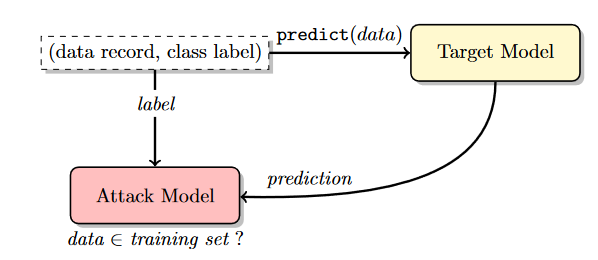
\includegraphics[width=0.5\textwidth]{TheorethicalFramework/AttacksOnPrivacy/shadow-models-mi.png}
  \caption{Black-box MIA attack on a machine learning model \citep{shokri_membership_2017}}
\end{figure}

Another approach to a black-box attack was introduced by Peng et al. and only considers that the attacker has access to the already trained model.
They first rescale the probabilities using temperature scaling to compensate for overconfident models \citep{peng_unsupervised_nodate}:
\begin{equation}
  R_i(h_k(x);T) = \frac{exp(log(h^i_k(x))/T)}{\sum_j{exp(log(h^j_k(x))/T)}}
\end{equation}
Here, the $h(x)$ denotes the probability distribution of $x$, which tells the chance of $x$ being a certain classification/label. Peng et al. then calculate the top-$k$ features $h_k$ and eliminate the smaller values.
The formula $R_i$ is the re-scaled probabilities, to be more suitable for clustering using temperature scaling, where $T$ is the scaling parameter.
They fit a K-Means model, resulting in two clusters: training and test data \citep{peng_unsupervised_nodate}.

\newpage

\section{Attack evaluation} \label{theory:attack-evaluation}
In this section, we evaluate the membership inference attack and evaluate it as it is the most appropriate for this study (See previous chapter).
We assess whether differential privacy provides protection against the attack and discuss how this can be measured.
\subsection{Member inference attacks}
% Research
Most current research for \gls{mia} is evaluated for neural networks \citep{rigaki_survey_2021}.
A tiny percentage evaluates this attack for supervised learning, with the majority using classification with decision trees.
Most studies have used a black-box approach \citep{rigaki_survey_2021} for these attacks.
This approach is not surprising, as these attacks have a high success rate and pose a greater risk of exploitation.

% Metrics
Introducing differential privacy reduces the impact of a member inference attack \citep{rigaki_survey_2021,hu_membership_2022}.
This is because the input to the model is perturbed.
While it is still possible to retrieve the training data, the leaked privacy is significantly reduced.
A simple but effective way to measure the privacy leakage is by calculating the accuracy of correctly predicting membership by the adversary \citep{choquette-choo_label-only_2021}.

Yeom et al. created a metric specifically for membership inference attacks which can be measured using an "adversarial advantage."
This metric describes the percentage of privacy compromised during a member inference attack \citep{yeom_privacy_2018}.
This metric is calculated by subtracting the \gls{fpr} from the \gls{tpr}.
The \gls{tpr} represents the number of correctly predicted member data (training data), and the \gls{fpr} represents the number of correctly predicted non-member data.
Although these metrics are commonly applied in the literature for \gls{mia}, they do not provide enough information \citep{carlini_membership_2022}.
Both metrics do not consider the imbalance between the \gls{tpr} and \gls{fpr}.
The metric should emphasize the \gls{tpr}, as this is the percentage of correctly predicted member data.
Therefore, they propose to use a ROC curve to show the effectiveness of a membership inference attack \citep{carlini_membership_2022}. \newline

% Final remark
In conclusion, the attacks that use \gls{mia} are all (mis)using supervised machine learning.
However, in this study, we use clustering algorithms.
Therefore, a semi-supervised approach can be used, as illustrated in Figure \ref{figure:MIA-semi-supervised}.
\newpage
\begin{figure}[h]
  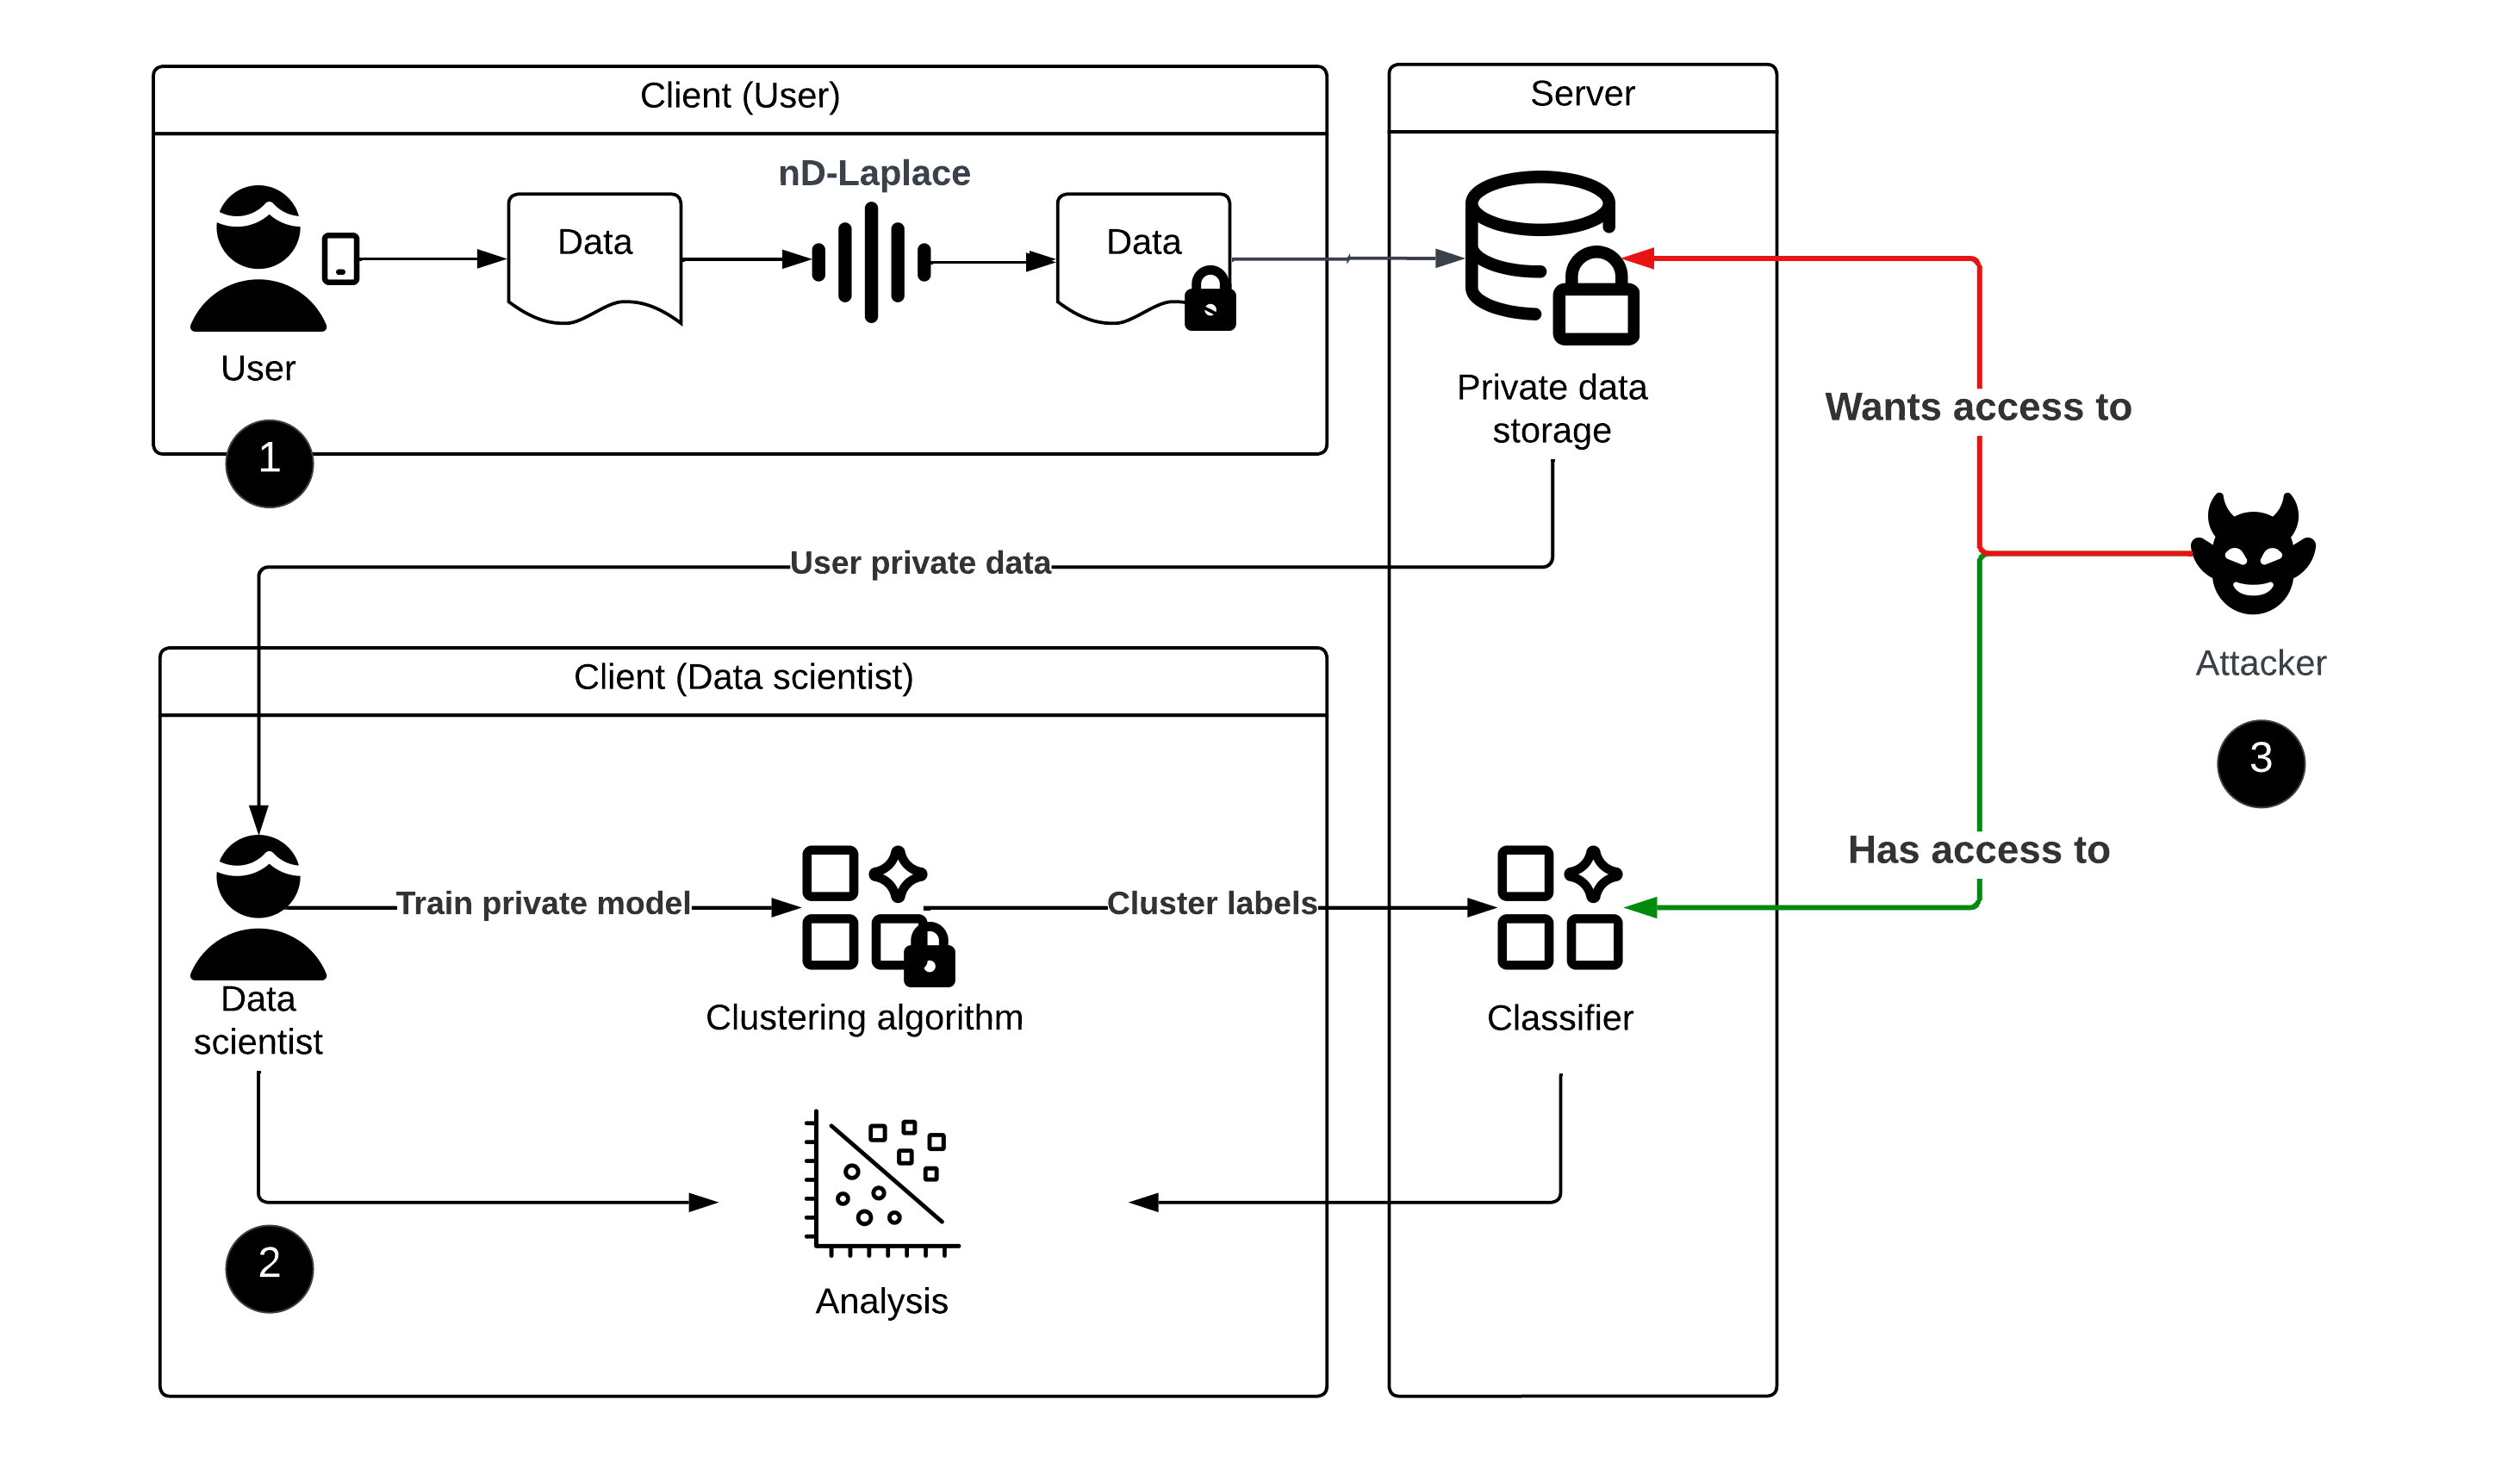
\includegraphics[width=1\textwidth]{TheorethicalFramework/Differential privacy/master-thesis-MIA.png}
  \caption{Semi-supervised black-box approach to execute a member inference attack.}
  \label{figure:MIA-semi-supervised}
\end{figure}

\begin{enumerate}
  \item The user uses a client (e.g., mobile app), where the nD-Laplace noise is added locally to the data.
  \item A data scientist trains the clustering algorithm with the privatized data.
        Therefore, the clustering algorithm's input and output (labels) are private.
        These labels are used to train a classifier (semi-supervised setup).
  \item The attacker wants access to the private data on the server.
        In this approach, the attacker has access to the classifier on the server (black-box setting).
        So, the attacker can use the classifier's output to conduct a \gls{mia}.
\end{enumerate}
